\documentclass[titlepage]{amsart}

\usepackage{amsmath,amssymb,amsthm,graphicx, paralist, appendix}


\usepackage{tabularx}
\usepackage{listings}
\usepackage{hyperref}
\usepackage{varioref}
\usepackage{subfigure}
\usepackage{amsrefs}
\usepackage[arrow, matrix, curve]{xy}
\usepackage{stmaryrd}
\usepackage{color}
\usepackage{mathrsfs}
\usepackage{bbold}
\usepackage[space]{grffile}

\usepackage{algorithm,algorithmic}

\hyphenation{english}
\hyphenation{mani-fold Wein-stein}

%%%%%%%%%%%% Commands   %%%%%%%%%%%%%%%%%%

\def\co{\colon\thinspace}
\newcommand{\Stein}{\mbox{\rm Stein}}
\newcommand{\Dim}{\mbox{\rm dim}}
\newcommand{\Div}{\mbox{\rm div}}
\newcommand{\im}{\mbox{\rm Im}}
\newcommand{\Int}{\mbox{\rm Int}}
\newcommand{\id}{\mbox{\rm id}}
\newcommand{\e}{\mathrm{e}}
\newcommand{\U}{\mathrm{U}}
\newcommand{\Diff}{\mathrm{Diff}}
\newcommand{\Cont}{\mathrm{Cont}}
\newcommand{\PD}{\mathrm{PD}}
\newcommand{\SO}{\mathrm{SO}}
\newcommand{\C}{\mathbb{C}}
\newcommand{\N}{\mathbb{N}}
\newcommand{\R}{\mathbb{R}}
\newcommand{\Z}{\mathbb{Z}}
\newcommand{\Q}{\mathbb{Q}}
\newcommand{\LL}{\mathbb{L}}
\newcommand{\oz}{\overline{z}}
\newcommand{\oL}{\overline{L}}
\newcommand{\oV}{\overline{V}}
\newcommand{\oW}{\overline{W}}
\newcommand{\ttt}{{\tt t}}
\newcommand{\tb}{{\tt tb}}
\newcommand{\tw}{{\tt tw}}
\newcommand{\otb}{\overline{\tt tb}}
\newcommand{\lk}{{\tt lk}}
\newcommand{\rot}{{\tt rot}}
\newcommand{\Deg}{{\tt deg}}
\newcommand{\fr}{{\tt fr}}
\newcommand{\cpk}{{\mathbb {CP}}^2}
\newcommand{\cpl}{{\mathbb {CP}}^1}
\newcommand{\rpk}{{\mathbb {RP}}^3}
\newcommand{\myparskip}{\parskip 4pt}


\newcommand{\com}[1]{\definecolor{Gray}{gray}{0.6}\noindent\textcolor{red}{\textit{#1}}}
\newcommand{\thought}[1]{--\textit{#1}--}
\newcommand{\note}[1]{
	\noindent
	\textcolor{black}{[[#1]]}
}
\newcommand{\MNote}[1]{\definecolor{Gray}{gray}{0.6}\textcolor{Gray}{}\marginpar{\textcolor{Gray}{Note: #1}}}

%%%%%%%%%%%% Theorems   %%%%%%%%%%%%%%%%%%

\newtheorem{thm}{Theorem}
\newtheorem*{thm*}{Theorem}
\newtheorem{lem}[thm]{Lemma}
\newtheorem{prop}[thm]{Proposition}
\newtheorem{cor}[thm]{Corollary}
\newtheorem{claim}[thm]{Claim}
\newtheorem*{claim*}{Claim}

\theoremstyle{definition}
\newtheorem{rem}{Remark}
\newtheorem*{rem*}{Remark}
\newtheorem*{rems*}{Remarks}
\newtheorem*{remdefn*}{Remark/Definition}
\newtheorem{defn}{Definition}
\newtheorem*{defn*}{Definition}
\newtheorem*{ex*}{Example}
\newtheorem{ex}{Example}
\newtheorem*{ack}{Acknowledgements}
\newtheorem*{que*}{Question}
\newtheorem{que}{Question}
\newtheorem*{ques}{Questions}
\newtheorem{alg}{Algorithm}
\newtheorem*{alg*}{Algorithm}



%------------------------------------------------------------------------------------------
%------------------------------------------------------------------------------------------
%------------------------------------------------------------------------------------------
%------------------------------------------------------------------------------------------
%------------------------------------------------------------------------------------------
\begin{document}


\title[]{The HTM Spatial Pooler as a Hopfield network}

%%%%%%%%%%%% Contact Info  %%%%%%%%%%%%%%%%%%

\author{Mirko Klukas}
\email{mirko.klukas@gmail.com}
\address[Mirko~Klukas]{Institute of Science and Technology Austria (IST Austria), 
Am Campus 1,
A – 3400 Klosterneuburg, Austria}
\date{\today}

%  
\begin{abstract}
These are \textbf{unfinished} notes!
My aim is to express Numenta's spatial pooler as a (constrained) Hopfield network.
In order to do so we have to express the \textit{w-max-overlap} procedure as
an appropriate energy function. This enables us to extend 
the energy by an additional term to decorrelate pairwise column activity
similar to P. Földiak's approach in his 1990's paper.

Relevant keywords are:
Hopfield networks, Boltzmann machines, Energy based models, Local anti-Hebbian learning by F\"oldi\'ak \cite{foldiak}.
% \begin{list}{-}{}
% \item Hopfield networks, 
% \item Boltzmann machines, 
% \item Energy based models, 
% \item Local anti-Hebbian learning by F\"oldi\'ak \cite{foldiak}
% \end{list}
See the references for relevant and more sources.
\end{abstract}
%
\maketitle
\tableofcontents
% 

% 
% =====================================================================
% =====================================================================
% 
\section{The Network}
% 
% =====================================================================
% =====================================================================
% 
% =====================================================================
% 
\subsection{Network architecture}
% 
% =====================================================================
% 
Let $m$ and $n$ be the number of visible and hidden units respectively. 
Furthermore we add a single bias unit, and connect all the units as follows. 
\begin{list}{}{}
\item[a.] \textbf{Visible-to-hidden} connections encoded by an $(n \times m)$-matrix $W$.
\item[b.] \textbf{Hidden-to-hidden} connections encoded by an $(n \times n)$-matrix $H$. 
          All hidden-to-hidden connections are symmetric without self connections,
          i.e. we have $h_{ji} = h_{ji}$, and $h_{ii} = 0$ for any $i,j$.
          (For the original spatial pooling algorithm these connections are zero.)
\item[c.] \textbf{Bias-to-hidden} connections encoded by a vector $b$ of size $n$ 
\end{list}
% 
\begin{figure}[h]
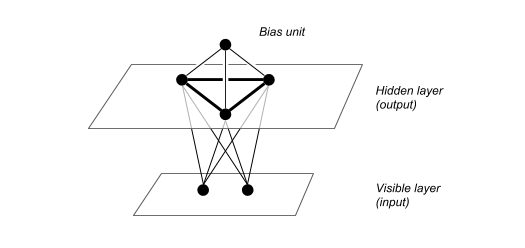
\includegraphics[width=0.6\textwidth]{./media/network_architecture_ebp.pdf}
\caption{Schematic picture of the network architeture.}
 \label{fig:network architecture}
\end{figure}
% 
% =====================================================================
% 
\subsection{Weight updates}
% 
% =====================================================================
% 
After each mini-batch the weights are updated and computed as follows:
The visible-to-hidden connections are updated according to a Hebbian-like update rule 
as described in \cite{sp_paper}, that is
% 
\begin{equation}
\label{eqn:numenta hebbian update}
\Delta w_{ij} = y_i \cdot  ( \varepsilon_+ \ x_j - \varepsilon_- \ \bar x_j ) 
\end{equation}
% 
After each update the visible-to-hidden connections
are clipped to be between $0$ and $1$, i.e. we set
% 
\begin{eqnarray*}
   &w_{ij} := 0& \text{ if } w_{ij} < 0 , \text{ and} \\
   &w_{ij} := 1& \text{ if } w_{ij} > 1.
\end{eqnarray*}
% 
The remaining connections - hidden-to-hidden and bias-to-hidden - 
are determined by the average activity of the hidden units as follows:
Let $\alpha_i$ denote the average activity of an individual unit $y_i$
(estimated by using an exponentially decaying average of the mean probability 
that a unit is active in each mini batch) then the weights of the bias 
connections are given by
% 
\begin{equation}
\label{eqn:bias update}
  b_{i}  = B_b \cdot \alpha_i.
\end{equation}
% 
Similar to the \textit{individual} average activity defined above we define 
the average \textit{pairwise} activity $\alpha_{ij}$ of two units $i$ and $j$.
With this in hand we set the hidden-to-hidden connections are given by
% 
\begin{equation}
\label{eqn:hidden updates}
  h_{ij} = B_H \cdot ( \alpha_{ij} - \alpha_i \ \alpha_j ) \ \text{ and } \  h_{ii} = 0.
\end{equation}
% 
Opionally we can clip $H$ to be non-negative, i.e.
$$
  h_{ij} := 0 \text{ if } h_{ij} < 0.
$$
Here $B_b$ and $B_H$ are two non-negative factors referred to as \textbf{boosting strength}.
% 
% =====================================================================
% =====================================================================
% 
\section{Energy function}
% 
% =====================================================================
% =====================================================================
% 
A straight-forward candidate for an energy function resembling the behaviour of 
the spatial pooler is
\begin{equation}
\label{eqn:numenta energy}
  E(x,y) = - \sum_{i=1}^n 
        y_i 
        \cdot
        \underbrace{
        \exp\Big( - b_i\cdot y_0 \ -  \sum_{j=1}^n h_{ij} \cdot y_j \Big)
        }_{\textit{"boosting"}}
        \cdot
        \underbrace{
        \Big(\sum_{j=1}^m w_{ij}\cdot x_j \Big)  
        }_{\textit{"overlap"}}
        \ + \  
        S(y)
\end{equation}
Here $S(y)$ denotes a \textit{size-penalty} (or \textit{size-bound}) forcing 
the weight of the vectors to be in a predefined desired range. 
For instance we could use something along the lines of
$$
    S(y) = 
    \begin{cases}
            0  &  \text{if $\|y\| \leq w$, and} \\
      +\infty  &  \text{otherwise,}
    \end{cases}
$$
where $w$ is a previously desired \textit{code weight} (that is, the number of active units).
% 
% =====================================================================
% =====================================================================
% 
\section{Encoding inputs}
% 
% =====================================================================
% =====================================================================
% 
The energy function $E$ defines a binary encoder by
$$
    \phi\colon \  x \mapsto \mathop{\arg\min}_y E(x,y).
$$
Note that the encoder associated with the above energy function does indeed 
extend the original \textit{spatial pooling procedure}: if we assume all the 
hidden-to-hidden connections to be zero, the above energy function does activate 
the units with the $w$-topmost \textit{boosted overlap scores}.
Note that in practice it is not feasible to compute the actual minimum, 
and we have to settle with the fact that we might only get to a local minimum.
% 
% =====================================================================
% =====================================================================
% 
\section{Questions}
% 
% =====================================================================
% =====================================================================
% 
\noindent\textbf{What are the advantages and disadvantages of the energy ``$E=e^A B$''?}
\parskip 5pt

...
\\

\noindent\textbf{What's the energy gap here?}
\parskip 5pt

See snippets...
\\

\noindent\textbf{What is the right way of finding an energy minimum?}
\parskip 5pt

Because the visible- to-hidden connections are clipped to be between 0 and 1 
the overlap scores are all positive. Further more the boosting term is also positive. 
Hence we are dealing with a special dynamic: assume $H \equiv 0$, and a uniform $b$, 
then the “radial direction” in $\{0,1\}^n$  is “gradient-like” for $E(x,.)$. 
In consequence if we start with a random $y$ of weight $w$ and do hill descend 
with neighbors at Hamming distance $1$ we are stuck. Note that if we start the 
hill descend at zero, and move in the direction of steepest descend, we end up 
with the $w$-topmost overlap scores. Alternatively we might add neighbours with 
the same weight at distance $2$, that is, allowing to switch an active unit off 
and an inactive one on.
% 
% =====================================================================
% =====================================================================
% 
\section{Local Anti-Hebbian learning after P. F\"oldi\'ak}
% 
% =====================================================================
% =====================================================================
% 
Here is a quick overview of the approach in \cite{foldiak}.
\textbf{A word of caution:} Please note that we are \textbf{NOT} using 
the notation from F\"oldi\'ak's paper here (in the paper $W$ denotes the 
hidden-to-hidden connections).
% 
% 
\subsection{Architecture and updates}
% 
% 
The architecture is similar to the one described above. The weight updates however 
are slightly different:
\begin{list}{}{}
\item[a.] \textbf{Visible-to-hidden} connections encoded by an $(n \times m)$-matrix $W$. 
          Updated according to (Hebbian update)
          $$
              \Delta w_{ij} = \varepsilon_W \ y_i \ (x_j - w_{ij}).
          $$
\item[b.] \textbf{Hidden-to-hidden} connections encoded by an $(n \times n)$-matrix $H$. 
          All hidden-to-hidden connections are symmetric without self connections. 
          Updated according to (anti-Hebbian update)
          $$
              \Delta h_{ij} = - \varepsilon_H\ ( y_i \ y_j - s^2).
          $$
          After any update the connections are clipped to be below $0$.
\item[c.] \textbf{Bias} or activation threshold encoded by a vector $b$ of size $n$. 
          Updated according to
          $$
              \Delta b = \varepsilon_B \ (y_i - s).
          $$
\end{list}
% 
Here $s \in [0,1]$ denotes a previouly fixed desired unit activation probability 
(I use $s$ indicating a \textit{sparse} activation probability).
% 
% 
\subsection{Encoding inputs}
% 
% 
(For a quick overview to this approach cf. for instance the scholarpedia article by 
Hopfield himself \cite{scholarpedia_hopfield}) To compute the hidden vector with a 
visible input clamped, we solve the following differential equation
$$
  \dot y_i = \sigma\big( W_i x + H_i y - b_i \big) - y_i.
$$
Here we treat $y_i$ as a \textit{continuous} variable.
\thought{It looks like the ODE computes a flowline (integral curve) of the energy gradient.} 
Actually, we are looking for a solution of the equation, but are interested in values
such that $\dot y_i = 0$.
Hence we are looking for a fixed point of
$$
f(p) = \sigma\big( Wx + Hp - b \big) .
$$
\thought{Recall that for the distribution associated to a Hopfield net we have
$P(y_i = 1 \ | \ x) = \sigma\big( W_i x + H_i y - b \big)$. So one would could
think of $y_i$ as the units activation probability.}


% 
% =====================================================================
% =====================================================================
% 
\section{Numenta's local inhibition revisited}
% 
% =====================================================================
% =====================================================================
% 
% 
Let us assume $h_{ij} \geq 0$ for now. Interpret 
the weights as a neighbourhood relationship. Informally a high weight
means ``being close'' and a high ``competitiveness'' between the corresponding units.
The situation described in \cite{sp_paper} would correspond to binary weights, 
i.e.\ either $h_{ij} = 0$ or $h_{ij} = 1$

We calculate a units activity $y_i$ as follows:
Turn the outgoing weights $h_{ij}$ for $i \neq j$ into 
an ``activation probability'' $a_{ij}$ by setting
\[
      a_{ij} := \frac{h_{ij}}{\mathop{\sum}\limits_{i \neq k} h_{ik} }.
\]
Informally this is a best guess for the activity of the other unit, assuming
unit $i$ is active.

With this in hand we calculate an estimate $A_i$ for the ``activation''
in the neighbourhood of unit $i$, i.e.\ we set
\[
    A_i = \mathop{\sum}\limits_{o_j > o_i} a_{ij}.
\]
Here $o_i$ denotes the \textit{boosted overlap score} of unit $i$ (that is $o_i = e^{-b} W_i x$).
The unit's score $o_i$ acts as a filter threshold to decide whose unit's ``activation'' it accumulates.
Note that we only accumulate the activity of units with a bigger overlap.
Then the \textbf{generalized local $w$-max procedure} can be expressed as
% 
\begin{equation}
\label{eqn:numenta unit activity}
      y_i = \begin{cases}
                1 & \text{if } A_i < s, \\
                0 & \text{otherwise}.
            \end{cases}
\end{equation}
% 
Here $s$ denotes a predefined desired sparsity $s = \tfrac{w}{n}$ ($w$ is the desired code weight). 
We can interpret this as follows: if the estimated activation is already bigger than desired,
i.e.\ bigger than the sparsity threshold $s$, we turn unit $i$ off. If it is smaller than
desired we turn unit $i$ on.
% 
\begin{rem*}
Further note that for binary weights this does indeed resemble Numenta's local $w$-max procedure,
because $A_i$ then is given by 
\[
  \mathop{\sum}\limits_{o_j > o_i} \tfrac{1}{n_i} = \tfrac{w_i}{n_i},
\]
where $n_i$ is the number of neighbours, and $w_i$ is the number of neighbours with a bigger overlap.
The condition $A_i < s$ would imply that $w_i < w$ which means that $o_i$ is among the $w$-biggest overlaps.
\end{rem*}
% 
%
%------------------------------------------------------------------------------------------
%------------------------------------------------------------------------------------------
%------------------------------------------------------------------------------------------
%------------------------------------------------------------------------------------------

\begin{thebibliography}{14}



\bibitem{foldiak}
\textsc{P.\ F\"oldi\'ak},
Forming sparse representations by local anti-Hebbian learning,
\textit{Biological Cybernetics} \textbf{64} (1990), 165--170.


\bibitem{sp_paper}
\textsc{Yuwei Cui, Subutai Ahmad, and Jeff Hawkins},
\textit{The HTM Spatial Pooler: a neocortical algorithm for online sparse distributed coding},
\texttt{bioRxiv:085035} (2017).


\bibitem{scholarpedia_hopfield}
\textsc{John J.\ Hopfield},
\textit{Hopfield network},
\text{http://www.scholarpedia.org/article/Hopfield{\_}network}.


\end{thebibliography}
%
%------------------------------------------------------------------------------------------
%------------------------------------------------------------------------------------------
%------------------------------------------------------------------------------------------
%------------------------------------------------------------------------------------------

%------------------------------------------------------------------------------------------
%------------------------------------------------------------------------------------------
%------------------------------------------------------------------------------------------
\end{document}

